\chapter{Umsetzung}

Dieses Kapitel dokumentiert den Aufbau der DML-Lautsprecher sowie deren Montage im Laborraum. Die Umsetzung basiert auf den Messergebnissen und Erkenntnissen aus Kapitel 3. Die fertiggestellten Lautsprecher verbleiben dauerhaft an ihrem Montageort und stehen für zukünftige Lehrveranstaltungen und Demonstrationszwecke zur Verfügung.

\section{Bau nach Testergebnissen}

Auf Grundlage der Versuchsergebnisse aus Kapitel 3 werden die Exciter an den simulativ ermittelten Positionen auf den Platten angebracht. Die Maße werden der technischen Zeichnung im Anhang J entnommen und auf den beiden 70 × 44 cm großen KAPA-Line-Platten angezeichnet. Da die asymmetrische Exciter-Positionierung ein asymmetrisches Abstrahlfeld erzeugt, werden die beiden Platten spiegelsymmetrisch zur mittleren Hochachse aufgebaut, um ein ausgewogenes Stereo-Klangbild zu erreichen.


\begin{figure}[H]
	\centering
	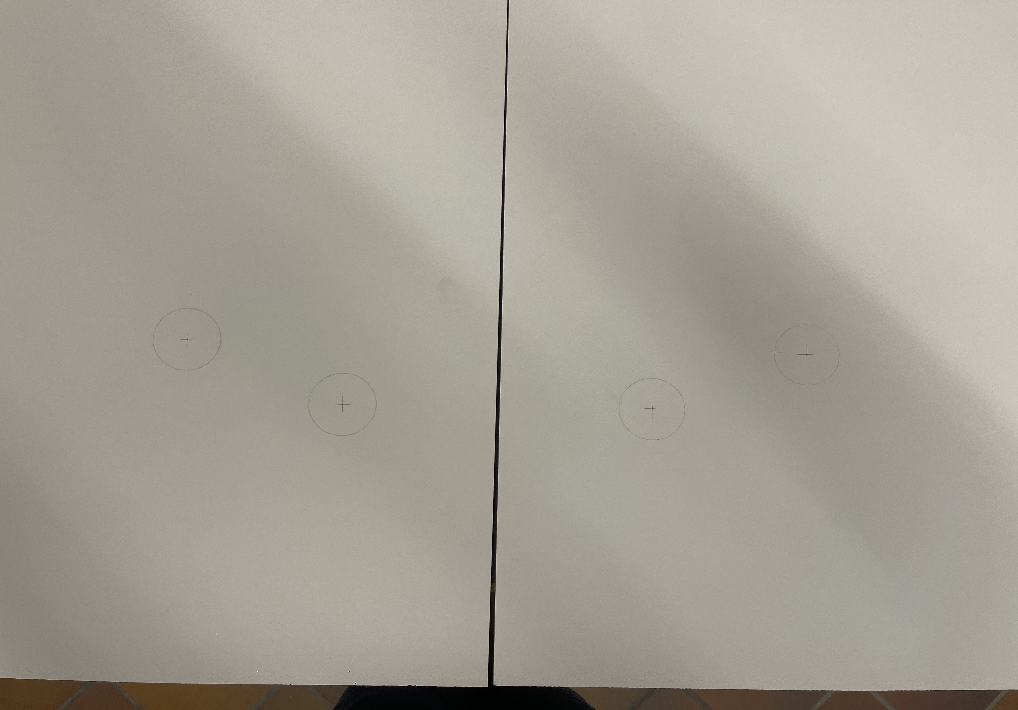
\includegraphics[width=0.8\textwidth]{pictures/DML_Exciterpostion.png}
	\caption{Angezeichnete Exciterpositionen auf den DML-Platten}
	\label{fig:exciterposition}
\end{figure}

Abbildung \ref{fig:exciterposition} zeigt die mit Bleistift auf der Plattendeckschicht angezeichneten Exciter-Positionen. Da die bereits im Versuchsaufbau verwendeten Exciter wiederverwendet werden, muss deren Klebefläche erneuert werden. Dazu wird die Kontaktfläche zunächst vom alten Kleber gereinigt und anschließend mit doppelseitigem Tesa-Klebeband neu beschichtet (siehe Anhang K). Die Lautsprecherkabel (Anhang L) werden an den Excitern in Reihenschaltung verlötet, um die gewünschte Gesamtimpedanz von 8 $\Omega$ zu erreichen. Beide Vorbereitungsschritte sind in Abbildung \ref{fig:klebeschicht_reihenschaltung} dargestellt.

\begin{figure}[H]
	\centering
	\includegraphics[width=0.6\textwidth]{pictures/Klebeschicht und Reihenschaltung Exciter.png}
	\caption{Neue Klebeschicht und verlötete Reihenschaltung der Exciter}
	\label{fig:klebeschicht_reihenschaltung}
\end{figure}

Abbildung \ref{fig:klebeschicht_reihenschaltung} zeigt im oberen Bereich die erneuerte Klebeschicht mit doppelseitigem Tesa-Klebeband sowie im unteren Bereich die verlötete Reihenschaltung der jeweils zwei Exciter pro Platte. Das Verbindungskabel zwischen den Excitern wurde auf 9 cm zugeschnitten, was dem Abstand zwischen den beiden Exciter-Positionen auf der Platte entspricht. Diese Kabellänge wurde bewusst kurz gewählt, damit das Kabel bei der Schwingungsanregung nicht gegen die Platte schlagen kann.


Für die Aufhängung der Platten hat sich im Schallfeldversuch die Methode mit eingeklebten Splinten bewährt. An den oberen Ecken der Sandwichplatten werden daher jeweils 2 cm vom Rand entfernt Splinte (Anhang N) mit UHU POR Kleber (Anhang O) eingeklebt. Die Platten werden anschließend frei hängend von der Decke montiert.

Als Befestigungslösung dient ein Nylonfaden (Anhang P), der in einen eigens konstruierten 3D-gedruckten Deckenhalter aus PLA (Anhang Q) eingeführt wird. Der Halter greift hinter die Leisten der Zwischendecke und klemmt sich dort zusammen mit dem Deckenpanel fest. Mit einer maximalen Traglast von 5 kg pro Nylonfaden ergibt sich bei zwei Fäden pro Platte eine Gesamttragfähigkeit von 10 kg. Da die Platten mit aufgeklebten Excitern lediglich etwa 1 kg wiegen, ist ein Sicherheitsfaktor von 10 gewährleistet.


\begin{figure}[H]
	\centering
	\includegraphics[width=\textwidth]{pictures/DML Aufgehängt.png}
	\caption{Aufgehängte DML-Lautsprecher im Laborraum}
	\label{fig:dml_aufgehaengt}
\end{figure}

Abbildung \ref{fig:dml_aufgehaengt} zeigt die fertig montierten DML-Lautsprecher, die im gleichen Abstand zur Wand angebracht wurden. Die Lautsprecherkabel werden durch einen Kabelkanal hinter der Platte geführt und oberhalb der Hängedecke verlegt. Dort erfolgt die Verbindung mit den zur Stereoanlage führenden Kabeln über litzengeeignete WAGO-Klemmen (Anhang N).

Die Kabelführung endet am Schaltschrank, in dem sich der Vorverstärker und der Equalizer befinden. Das Audiosignal wird über ein AUX-Kabel in den Equalizer eingespeist, von dort über ein Cinch-Kabel an die Leistungsendstufe weitergeleitet und schließlich an die DML-Lautsprecher ausgegeben. Die vollständige Verkabelung der Audiokomponenten ist in Abbildung \ref{fig:verkabelung_stereoanlage} dargestellt. 


\begin{figure}[H]
	\centering
	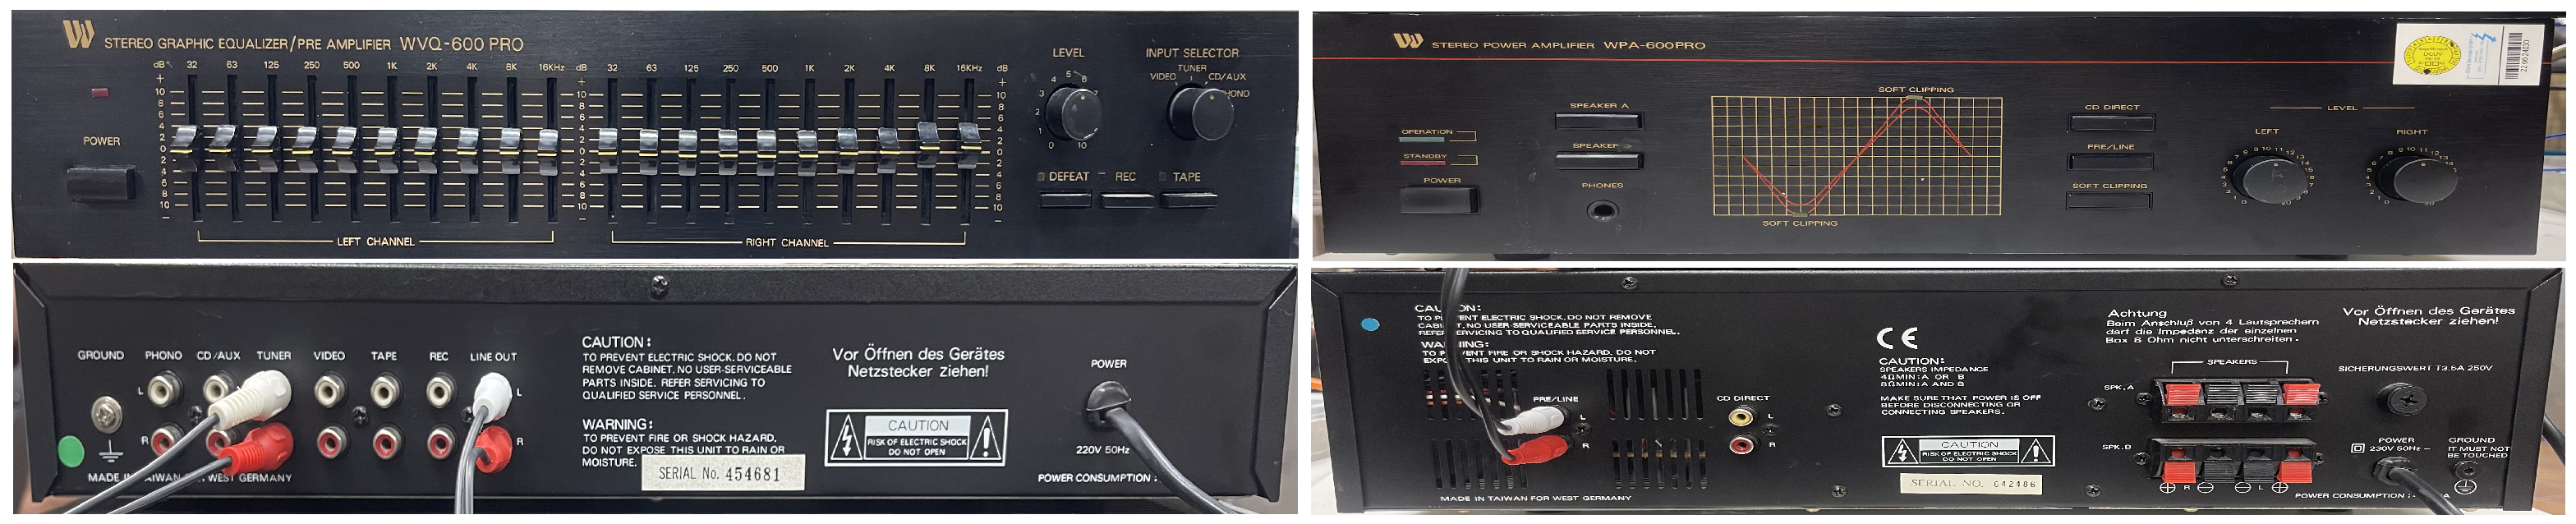
\includegraphics[width=\textwidth]{pictures/Kabel_Stereoanlage.png}
	\caption{Verkabelung der Stereoanlage mit Vorverstärker und Equalizer}
	\label{fig:verkabelung_stereoanlage}
\end{figure} 


\section{Subjektive Hörvalidierung}

Da im Laborraum keine Messtechnik zur akustischen Analyse vorhanden ist, erfolgte die Validierung der fertig montierten DML-Lautsprecher ausschließlich auf subjektiver Basis. Dabei wurden verschiedene Musiktitel unterschiedlicher Genres wiedergegeben und hinsichtlich ihrer Klangqualität beurteilt.

Bei der Wiedergabe von Musik mit ausgeprägtem Mittel- und Hochtonanteil, wie beispielsweise Gesang und akustische Instrumente, zeigten die DML-Lautsprecher eine angenehme räumliche Wiedergabe mit breiter Bühnenabbildung. Die für DML-Systeme typische diffuse Abstrahlung führte zu einem umhüllenden Klangeindruck, der insbesondere bei Hintergrundmusik als angenehm empfunden wurde.

Im Tieftonbereich waren die erwarteten Einschränkungen wahrnehmbar. Bassintensive Musikstücke klangen zunächst weniger druckvoll. Durch Anpassung des Equalizers konnte der Klangeindruck subjektiv verbessert werden. Die Equalisation erfolgte dabei rein nach Gehör, da keine messtechnische Unterstützung zur Verfügung stand. Diese Vorgehensweise ist kritisch zu betrachten, da sie stark von der individuellen Wahrnehmung und den akustischen Gegebenheiten des Raumes abhängt. Eine objektive Reproduzierbarkeit der Einstellungen ist somit nicht gewährleistet.

Es ist davon auszugehen, dass durch eine messtechnisch gestützte Abstimmung, beispielsweise mittels Raumeinmessung und frequenzselektiver Korrektur, ein deutlich verbessertes akustisches Ergebnis erzielt werden könnte. Dies stellt einen möglichen Ansatzpunkt für zukünftige Optimierungen dar.

\subsection{Ergebnisdiskussion}



